\documentclass[a4paper,UTF8]{article}
\usepackage{ctex}
\usepackage[margin=1.25in]{geometry}
\usepackage{color}
\usepackage{graphicx}
\usepackage{amssymb}
\usepackage{amsmath}
\usepackage{amsthm}
\usepackage{enumerate}
\usepackage{bm}
\usepackage{hyperref}
\usepackage{pgfplots}
\usepackage{epsfig}
\usepackage{color}
\usepackage{tcolorbox}
\usepackage{mdframed}
\usepackage{lipsum}
\usepackage{framed}
\usepackage{setspace}

\newmdtheoremenv{thm-box}{myThm}
\newmdtheoremenv{prop-box}{Proposition}
\newmdtheoremenv{def-box}{定义}

\setlength{\evensidemargin}{.25in}
\setlength{\textwidth}{6in}
\setlength{\topmargin}{-0.5in}
\setlength{\topmargin}{-0.5in}
% \setlength{\textheight}{9.5in}
%%%%%%%%%%%%%%%%%%此处用于设置页眉页脚%%%%%%%%%%%%%%%%%%
\usepackage{fancyhdr}                                
\usepackage{lastpage}                                           
\usepackage{layout}                                             
\footskip = 10pt 
\pagestyle{fancy}                    % 设置页眉                 
\lhead{2023年秋季}                    
\chead{数字信号处理}                                                
% \rhead{第\thepage/\pageref{LastPage}页} 
\rhead{作业二}                                                                                               
\cfoot{\thepage}                                                
\renewcommand{\headrulewidth}{1pt}  			%页眉线宽,设为0可以去页眉线
\setlength{\skip\footins}{0.5cm}    			%脚注与正文的距离           
\renewcommand{\footrulewidth}{0pt}  			%页脚线宽,设为0可以去页脚线

\makeatletter 									%设置双线页眉                                        
\def\headrule{{\if@fancyplain\let\headrulewidth\plainheadrulewidth\fi%
\hrule\@height 1.0pt \@width\headwidth\vskip1pt	%上面线为1pt粗  
\hrule\@height 0.5pt\@width\headwidth  			%下面0.5pt粗            
\vskip-2\headrulewidth\vskip-1pt}      			%两条线的距离1pt        
 \vspace{6mm}}     								%双线与下面正文之间的垂直间距              
\makeatother  

%%%%%%%%%%%%%%%%%%%%%%%%%%%%%%%%%%%%%%%%%%%%%%
\numberwithin{equation}{section}
%\usepackage[thmmarks, amsmath, thref]{ntheorem}
\newtheorem{myThm}{myThm}
\newtheorem*{myDef}{Definition}
\newtheorem*{mySol}{Solution}
\newtheorem*{myProof}{Proof}
\newtheorem*{myRemark}{备注}
\renewcommand{\tilde}{\widetilde}
\renewcommand{\hat}{\widehat}
\newcommand{\indep}{\rotatebox[origin=c]{90}{$\models$}}
\newcommand*\diff{\mathop{}\!\mathrm{d}}

\usepackage{multirow}

%--

%--
\begin{document}

\title{数字信号处理\\
作业二}
\author{你的名字\, 你的学号} 
\maketitle
%%%%%%%% 注意: 使用XeLatex 编译可能会报错,请使用 pdfLaTex 编译 %%%%%%%

\section*{作业提交注意事项}
\begin{tcolorbox}
    \begin{enumerate}
        \item[(1)] 本次作业提交截止时间为~\textcolor{red}{\textbf{2023/11/13  23:59:59}},截止时间后不再接收作业,本次作业记零分;
        \item[(2)] 作业提交方式:使用此~LaTex~模板书写解答,只需提交编译生成的~pdf~文件,将~pdf~文件上传至https://box.nju.edu.cn/u/d/9e2a5f229a03407f9f86/;
        \item[(3)] pdf 文件命名方式:学号-姓名-作业号-v版本号, 例~ MG1900000-张三-1-v1;如果需要更改已提交的解答,请在截止时间之前提交新版本的解答,并将版本号加一;
        \item[(4)] 未按照要求提交作业,或~pdf~命名方式不正确,将会被扣除部分作业分数。

    \end{enumerate}
\end{tcolorbox}


\newpage
\section{[40pts] 系统微分方程的求解 }
求解以下微分方程所表示的系统的完全响应:
\begin{enumerate}[(1)]
    \item $y^{(3)}(t)-3y^{(1)}(t)+2y(t)=10\sin t$ $(t\geqslant0)$, 边界条件$y(0)=y^{(1)}(0)=y^{(2)}(0)=0$。
    \item $y[n]-\displaystyle\frac{1}{2}y[n-1]-y[n-2]+\frac{1}{2}y[n-3]=-2x[n]+2x[n-1]$,其中$x(n)=\displaystyle\left(\frac{1}{3}\right)^n$,边界条件$y(0)=y(-1)=0,y(-2)=1$。
\end{enumerate}

\begin{framed}
    \begin{spacing}{1.5}
        \begin{itemize}
            \item 你的解答。
        \end{itemize}
    \end{spacing}
\end{framed}


\newpage
\section{[20pts] 系统的响应 }
已知系统方程为$y^{(2)}(t)+6y^{(1)}(t)+8y(t)=4e^{-t}$且无跳变, 起始状态为$y(0_{-})=0,y^{(1)}(0_{-})=-4$.求系统的零输入响应和零状态响应。

\begin{framed}
    \begin{spacing}{1.5}
        \begin{itemize}
            \item 你的解答。
        \end{itemize}
    \end{spacing}
\end{framed}

\newpage
\section{[40pts] 傅里叶级数}
设$x(t)$为某一周期信号。
\begin{enumerate}[(1)]
	\item 设$x(t)$的部分图像如下所示:\\
	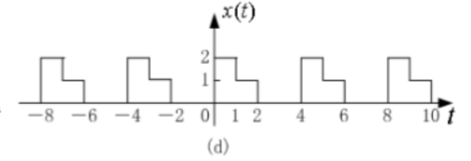
\includegraphics[scale=0.4]{1.png}\\
	求$x(t)$的\textbf{傅里叶级数}表达式。
	\item 设$x(t)$的基波周期为$T_0$,傅里叶级数的系数为$\dot{A}_k$,请用$\dot{A}_k$表示下列傅里叶级数的系数:\\
	(a) $x(t+t_0)$\\
	(b) $x(-t)$\\
	(c) $\displaystyle\int_{-\infty}^tx(\tau)d\tau$,假设$\dot{A}_0=0$\\
	(d) $\displaystyle\frac{dx(t)}{dt}$
\end{enumerate}

\begin{framed}
\begin{spacing}{1.5}
    \begin{itemize}
    \item 你的解答。
    \end{itemize}
\end{spacing}
\end{framed}


\newpage
\end{document}